\subsection{Exam: 2022. 06. 13., Exercise 2}

\lineparagraph{Exercise}

We would like to create a single tape, \textbf{deterministic} Turing-machine, that recognizes the language $L=a(a+b+c)*bc$. On the following diagram, we can see the Turing-machine's structure, with missing transitions, labeled $t_1, t_2, t_3, t_4, t_5$. Give the transitions, so that the Turing-machine recognizes $L$ and explain how the machine works!($t_1, t_2$ and $t_3$ are parallel edges in the TM.)

\begin{center}
    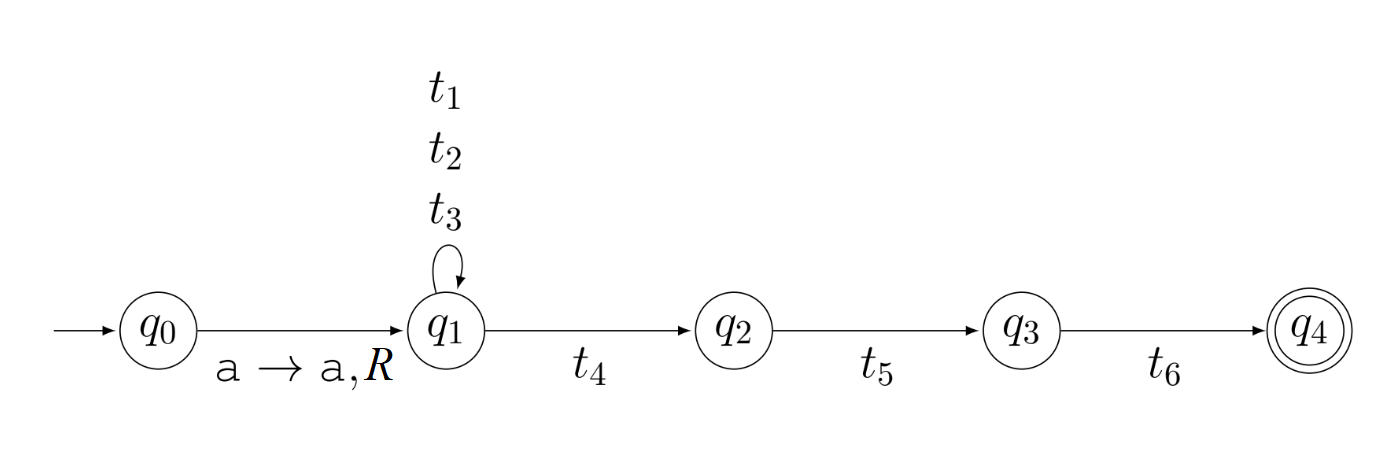
\includegraphics[width=0.8\linewidth]{exams/2022_06_13/02/tm.png}
\end{center}

\lineparagraph{Solution}

\begin{itemize}
    \item The $q_0 \rightarrow q_1$ transition makes sure that the first $a$ character from $L=a(a+b+c)^*bc$ is present.
    \item The $t_1, t_2, t_3$ loop is important, because that's the only way we can deal with the $*$ operator on $(a+b+c)^*$. The loop can execute any number of times (including zero), similarly the star operator means the inner part can be repeated any number of times (including zero).
    \item Inside $(a+b+c)^*$, we have $a+b+c$, which means either $a$, or $b$ or $c$ character is present.
    \item The loop is allowed to have $3$ transitons, so we can use $1$ transition to deal with one of the three characters.
    \item So $t_1 = a \rightarrow a, R$, $t_2 = b \rightarrow b, R$, $t_3 = c \rightarrow c, R$. It is important to move the head to the right, otherwise we would be stuck in the same place, reading in the same character over and over again, resulting in an infinite loop, which would mean the TM rejects the input word and we don't want that.
    \item Finally, we need to make sure that the word ends in $bc$, since $L=a(a+b+c)^*bc$.
    \item This part many people wrote $t_4 = b \rightarrow b, R$. Unfortunately, this is incorrect, because it collides with the $t_2$ transition. Both $t_2$ and $t_4$ can be executed when the head sees a $b$ character on the tape, resulting in nondeterministic behaviour. The task asked to give a deterministic Turing-machine, so this is not good.
    \item Instead, we are going to allow the $t_2$ and the $t_3$ transition to read the $b$ and $c$ at the end of the word in. While we cannot guarantee at this point that the word actually ended in $b$ and $c$, the $t_1$, $t_2$ and $t_3$ transitions will move the head past whatever characters are at the end, until we see a $*$ on the tape.
    \item We are going to use $t_4$ to detect this $*$, so $t_4 = * \rightarrow *, L$. We are moving to the left here, because we want to go back and make sure the word ends in $bc$.
    \item Now we will encounted the ending $c$ character first, so $t_5 = c \rightarrow c, L$.
    \item Finally we make sure the previous character is $b$, so $t_6 = b \rightarrow b, L$.
\end{itemize}

